\documentclass[a4paper]{scrartcl}

%% Language and font encodings
\usepackage{newfloat}

\usepackage{wrapfig}
\usepackage{listings}
\usepackage[english]{babel}
\usepackage[utf8]{inputenc}
\usepackage[T1]{fontenc}
\usepackage{tikz}
\usepackage{indentfirst}
\usetikzlibrary{shapes,arrows}

\usepackage{subfigure}
\usepackage[newfloat]{minted}
% \captionsetup[listing]{position=top}
\usepackage[backend=biber,style=authoryear]{biblatex}
\usepackage{lmodern}
\addbibresource{Mendeley.bib}
% \usepackage{floatrow}

%% Sets page size and margins
% \usepackage[a4paper,top=2.5cm,bottom=2cm,left=3cm,right=3cm,marginparwidth=1.75cm]{geometry}

%% Useful packages
\usepackage{algpseudocode}
\usepackage{enumitem}
\usepackage{amsmath}
\usepackage{graphicx}
\usepackage{multicol}
\usepackage[colorinlistoftodos]{todonotes}
\usepackage[colorlinks=true, allcolors=blue]{hyperref}
\renewcommand{\thesubfigure}{\thefigure.\arabic{subfigure}}
\newcommand{\ttt}[1]{\texttt{#1}}

%% Tikz
\tikzstyle{decision} = [diamond, draw, 
    text width=6.5em, text badly centered, node distance=3cm, inner sep=0pt]
\tikzstyle{block} = [rectangle, draw, 
    text width=5em, text centered, minimum height=4em]
\tikzstyle{line} = [draw, -latex']
\tikzstyle{cloud} = [draw, ellipse, node distance=3cm,
    minimum height=2em]
    
    
\begin{document}
\title{Documentation Localization \& Navigation}
\author{Xinrui Li}
\maketitle
\section{Localization}
We use a bag of words approach for localization.
\subsection{Learning and Constructing the Dictionary}

\textbf{Terminology}:
\begin{enumerate}
\item \textbf{Feature} Interest point in the image, for example a SIFT descriptor.
\item \textbf{Word} A ball in the feature space.
\item \textbf{Node} A node in the tree structure, can store a number of words.
\end{enumerate}

\begin{listing}[H]
\caption{Learning equals memorizing labels.}
\begin{minted}[frame=single,obeytabs=true,tabsize=4]{matlab}
function LearnImage(image, label, dict)
	SIFTFeatures = SIFT(image);
    for feature in SIFTFeatures
    	%words are actually balls in feature space
		AddFeatureToDict(feature, label, dict);
    end
end
\end{minted}
\end{listing}

\begin{listing}[H]
\caption{AddFeatureToDict(feature, label, dict) adds label to the words that contains the feature.}
\begin{minted}[frame=single,obeytabs=true,tabsize=4]{matlab}
function AddFeatureToDict(feature, label, dict)
	%Adding feature to dict
	%Find words in the dict that contains feature
	wordList = Search(feature, dict) % Filliat 08
    %Add feature to existing words or create a new word
    if (wordList != NULL) % Found existing words
    	for word in wordList
        	UpdateWord(label, word) 
		end
    else % no existing word
    	[word, node] = AddNewWord(feature, dict) 
        UpdateWord(label, word)
        
        %Adjusting dict structure if a node has too many words
        if (node.ChildrenCount > NUM_CHILDREN_MAX)
            %Split its children words into k leaf nodes
            [centers] = KMeansCluster(k, node.words)
			for center in centers
            	newNode = AddNewNode(center)
                AddParentNode(newNode, node)
            	AddWordToNode(center.words, newNode)
                RemoveWordFromNode(center.words, node)
    		end
        end
    end
end
\end{minted}
\end{listing}

\subsection{Identifying}
\begin{listing}[H]
\caption{Identify(imageCollection) does a two-level vote. }
\begin{minted}[frame=single,obeytabs=true,tabsize=4]{matlab}
function Identity(imageCollection)
	numImage = 0
	firstLevelVote = []
	for image in imageCollection   	
    	numImage += 1
        %Use multiple feature spaces, like SIFT, color histogram
        wordCollection = []
        for FeatureMethod, dict in [FEATURE_METHODS, dicts]
            features = FeatureMethod(image)
            for feature in features
                wordList = Search(dict, feature)
                wordCollection = [wordCollection, wordList]
                % Words vote by inverse document frequency for room label
                [room, quality] = FirstVoteIdf(wordList)
                % quality mesured by difference of scores
                if quality > THRESHOLD_QUALITY_FIRST
                    firstLevelVote = [firstLevelVote, room]
                end
            end
        end 
        
        [result, quality] = SecondVote(firstLevelVote)
        if quality > THRESHOLD_QUALITY_FIRST 
         	% Success, add labels to words 
            for word in wordCollection
            	UpdateWord(label, word)
            end
        elseif (numImage > NUM_IMAGE_MAX)
        	return -1; % unidentified
        end        
  	end
end
\end{minted}
\end{listing}

\subsection{Local Color Histogram}
The image is decomposed in a
set of overlapping windows of several sizes in order to
provide some scale invariance. The histograms of the
H value in the HSV color space for each window are
used as features. The windows used are of size 40x40
pixels taken each 20 pixels and 20x20 pixels taken each
10 pixels. The descriptors are of dimension 16 and are
compared using diffusion distance [27].
\begin{listing}[H]
\caption{Calculation of Local Color Histogram Distance}
\begin{minted}[frame=single,obeytabs=true,tabsize=4]{matlab}
function CalculateFeatures(img)
	imgWindows = GetWindows(img)
    features = []
    for window in imgWindows
    	hue = GetHueChannel(window)
        hist = CalcHist(window, nBins = 16)
        features = [features, hist]
    return features
\end{minted}
\end{listing}

\subsection{Searching Features}
\begin{figure}[H]
\centering
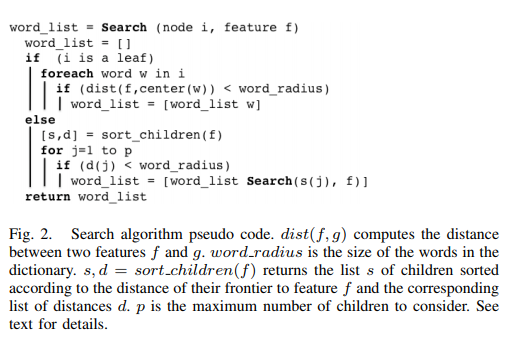
\includegraphics[width = 0.8\textwidth]{img/search.png}
\caption{\ttt{Search} Function in Filliat 08}
\end{figure}

\newpage
\section{Topological Cartography}

\subsection{Room Level}
In the first step, we can create a simple map for rooms and their connections during learning.

\begin{listing}[H]
\caption{Creating room map}
\begin{minted}[frame=single,obeytabs=true,tabsize=4]{matlab}
function LearnRoomMap()
	(during learning)
    if (currentRoom != lastRoom)
    	AddRoomConnection(currentRoom, lastRoom)
\end{minted}
\end{listing}

This is a very straightforward method, but it requires the robot / user to take a photo each time it passes a room, even if it is a familiar one.

\subsection{Landmarks inside Rooms}
The next step is to enable the robot to navigate between rooms as well as inside rooms. We would have for each room several landmarks, some leading to other rooms are seen as key landmarks. When the robot needs to enter another room than the current, it will first go to a key landmark (with the right orientation), then advance until localization result changes to the new room.

The robot should be capable of:
\begin{enumerate}
\item Localize itself with respect to landmarks. Either it is exactly at one landmark, or it can know its distance and angle to the landmarks present in the room.
\item Navigate toward landmarks. With its knowledge of the environment obtained in the last step and information provided by odometry, it should be able to go to one assigned landmark. 
\end{enumerate}

We would like to use RGB-D camera for navigation and detection of doors, passages as well as distances between landmarks etc.

It is also worth noting that we assume for the moment there is no big obstacles present in the room, and once given orientation and distance to the goal the navigation would be rather easy. 

\subsection{Calculation of Orientation}
Algo: one landmark consists of N images taken at the same spot in a circle. Then given an image, we can calculate the angle with respect to this landmark.
%TODO: plot an diagram.

\subsection{Calculation of Distance}
% For the moment, we don't have a reliable odometry on Buddy, and we don't have a RGB-D camera neither. So we won't consider distance for the moment.

\subsection{Navigation toward the goal}
For each room, we will have "Key Landmarks" that lead to    

\newpage
\section{Scenario}
In this section we describe a general scenario in which the user will take Buddy (the robot) around his home, while the robot will learn the rooms as well as build a topological map. 

Upon entering a new room, the user can choose to set up a landmark or simply learn one image. If the former, the robot will take a series of photos while rotating, ensuring that it can recognize this landmark in any orientation. If the latter, it will simply learn an image as described in section one. The user can also declare a key landmark, or it is also possible that the robot can detect this itself. 

Once finished, the robot enters the next room, while adding the connection between these two rooms. As mentioned earlier, if the robot passes by a familiar room to a new room, it should learn at least once in the familiar room so that the algorithm can establish the correct connections.

\section{Problems}
\subsection{Non-Symmetric Order issues}
During experimentation, we have found that sometimes the order in which the rooms are learned can influence the resulting dictionary, consequently localization precision.

To illustrate this, we run the training algorithm on two rooms: cuisine and reunion. In experiment 1, we train first on cuisine then on reunion, and vice versa in experiment 2. SIFT descriptors are used, and hyperparameters remain the same across two experiments. It turns out that the correct rate is very low in the second case. ($ \textit{MAX\_CHILD\_NUM} = 1$)

\begin{table}[H]
\centering
\caption{Correct and unidentified rate in two experiments}
\label{rates_nonsym}
\begin{tabular}{l l l}
\hline
        & Cuisine        &   Reunion      \\ \hline
Experiment 1 (Cuisine first)   & 100\% / 0\% & 95.65\% / 0\% \\ \hline
Experiment 2 (Reunion first) &  100\% / 0\% & 20\% / 50\% \\ \hline
\end{tabular}
\end{table}

% \begin{table}[H]
% \centering
% \caption{Correct and unidentified rate in two experiments}
% \label{rates_nonsym}
% \begin{tabular}{l l l}
% \hline
%         & Salon        &   Cuisine      \\ \hline
% Experiment 1 (Salon first)   & 89.47\% / 10.53\% & 100\% / 0\% \\ \hline
% Experiment 2 (Cuisine first) &  100\% / 0\% & 64.7\% / 11.76\% \\ \hline
% \end{tabular}
% \end{table}

The dictionaries built in the two experiments contain different number of words for the two rooms. There are more words associated to one room if it is learned later. 
\begin{table}[H]
\centering
\caption{SIFT word statistics for two experiments}
\label{words_sym}
\begin{tabular}{|l|l|l|l|l|}
\hline
             & Total Words & Cuisine & Reunion & Shared \\ \hline
Experiment 1 & 10407       & 5578    & 5015    & 186    \\ \hline
Experiment 2 & 10421       & 5848    & 4748    & 175    \\ \hline
\end{tabular}
\end{table}


We show this in the following diagram. Here we have three features, green ones for room A, yellow ones for room B. (In our case A is Cuisine and B is reunion) The numbers above features are the sequence in which they are learned. In case one A's features are learned first, so when feature 3 is learned, word 2 will be created but the fact that 2 is also in it will be ignored. On the contrary, in case 2 when B is learned beforehand, feature 3 will also be added to word 2.

\begin{figure}[H]
\caption{Illustration on different dictionaries caused by learning order}
\vskip 5pt
\tikzset{every picture/.style={line width=0.75pt}} %set default line width to 0.75pt        
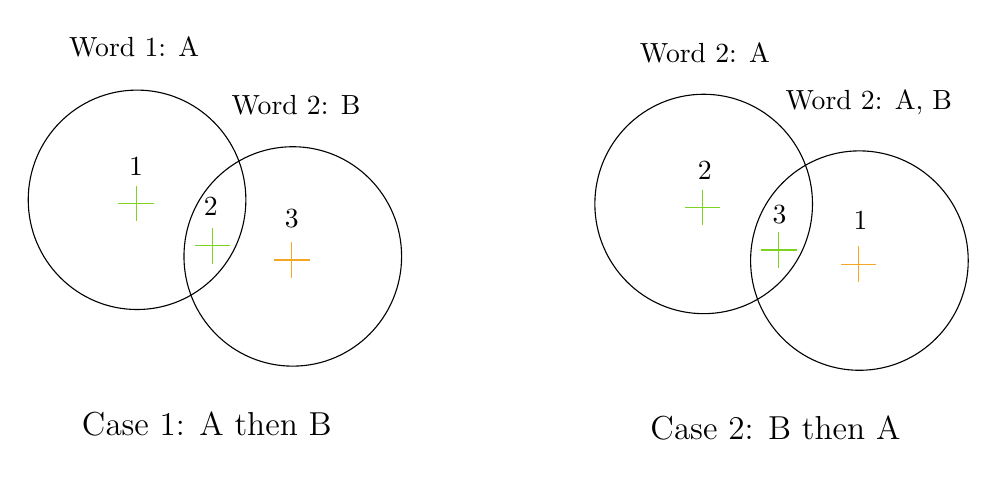
\begin{tikzpicture}[x=0.75pt,y=0.75pt,yscale=-1,xscale=1]
%uncomment if require: \path (0,300); %set diagram left start at 0, and has height of 300
\draw    (163.43, 138.86) circle [x radius= 52.43, y radius= 52.86]  ;
\draw  [color={rgb, 255:red, 126; green, 211; blue, 33 }  ,draw opacity=1 ] (154.48,140.56) -- (171.53,140.56)(163.01,132.04) -- (163.01,149.09) ;
\draw    (238.46, 166.14) circle [x radius= 52.43, y radius= 52.86]  ;
\draw  [color={rgb, 255:red, 245; green, 166; blue, 35 }  ,draw opacity=1 ] (229.51,167.85) -- (246.56,167.85)(238.03,159.32) -- (238.03,176.37) ;
\draw  [color={rgb, 255:red, 126; green, 211; blue, 33 }  ,draw opacity=1 ] (191.14,161.03) -- (208.19,161.03)(199.67,152.5) -- (199.67,169.55) ;
\draw    (436.43, 140.86) circle [x radius= 52.43, y radius= 52.86]  ;
\draw  [color={rgb, 255:red, 126; green, 211; blue, 33 }  ,draw opacity=1 ] (427.48,142.56) -- (444.53,142.56)(436.01,134.04) -- (436.01,151.09) ;
\draw    (511.46, 168.14) circle [x radius= 52.43, y radius= 52.86]  ;
\draw  [color={rgb, 255:red, 245; green, 166; blue, 35 }  ,draw opacity=1 ] (502.51,169.85) -- (519.56,169.85)(511.03,161.32) -- (511.03,178.37) ;
\draw  [color={rgb, 255:red, 126; green, 211; blue, 33 }  ,draw opacity=1 ] (464.14,163.03) -- (481.19,163.03)(472.67,154.5) -- (472.67,171.55) ;

\draw (163,123) node  [align=left] {1};
\draw (199,142) node  [align=left] {2};
\draw (238,148) node  [align=left] {3};
\draw (437,125) node  [align=left] {2};
\draw (473,146) node  [align=left] {3};
\draw (512,149) node  [align=left] {1};
\draw (162,65) node  [align=left] {Word 1: A};
\draw (240,93) node  [align=left] {Word 2: B};
\draw (437,68) node  [align=left] {Word 2: A};
\draw (516,92) node  [align=left] {Word 2: A, B};
\draw (197,247) node  [align=left] {{\fontfamily{helvet}\selectfont {\large Case 1: A then B}}};
\draw (471,249) node  [align=left] {{\large Case 2: B then A}};
\end{tikzpicture}

\end{figure}
In the end, this non-symmetrical learning can degrade the performance of our model. 

\subsection{Solution to order-dependent learning}
To address this problem, we have conceived an \textit{ad hoc} solution. During learning, when a new feature is added to an existing word $w$, the feature itself will be stored along with its label. Thus, when a new word $w'$ whose center is less than $2 R$ ($R$ is the radius of a word) to $w$ is created, the old features stored in $w$ will be re-passed to $w'$. Therefore, as in case one, when word 2 is created, feature 2 will also be added to word 2, so it will end up having both labels A and B.

\begin{table}[H]
\centering
\caption{Correct and unidentified rate in two experiments, with feature review}
\label{rates_sym}
\begin{tabular}{l l l}
\hline
        & Cuisine        &   Reunion      \\ \hline
Cuisine first   & 100\% / 0\% & 85.71\% / 14.29\% \\ \hline
Reunion first &  100\% / 0\% & 69.23\% / 7.69\% \\ \hline
\end{tabular}
\end{table}

% \begin{table}[H]
% \centering
% \caption{Speed comparison}
% \label{rates_sym}
% \begin{tabular}{l l l}
% \hline
%         &  k=1  &   k=3     \\ \hline
% Before   & 98ms  & 251ms \\ \hline
% After & 115ms  & 311ms \\ \hline
% \end{tabular}
% \end{table}

\begin{table}[H]
\centering
\caption{SIFT word statistics for two experiments}
\label{words_sym}
\begin{tabular}{|l|l|l|l|l|}
\hline
             & Total Words & Cuisine & Reunion & Shared \\ \hline
Experiment 1 & 10407       & 5644    & 5015    & 252    \\ \hline
Experiment 2 & 10421       & 5848    & 4837    & 246   \\ \hline
\end{tabular}
\end{table}

From test results we can see that the correct rate for reunion has increased from 20\% to nearly 70\% with feature review. Meanwhile, the average time for processing one image during localization has increased from 98ms to 112ms, which is rather acceptable. 

On the other hand, one shortcoming of this solution is that it will require more memory. Before we only have to store the center of words, now it is necessary to store all the features, which can be two times memory-consuming with the current hyperparameters.

\subsection{Binary / K-Means}
Due to the fact that SIFT and SURF image descriptors are patent protected, we are obliged to experiment with other image descriptors. Many of the these are binary descriptors, like FREAK, ORB and BRISK. However, when using these binary descriptors together with the Hamming distance, we can have some terrible correct rates. 

After some reflection, I came to realize that this is caused by the k-means step during bag-of-words dictionary construction. For continuous valued vectors, using their mean as the centroid makes sense, but this is not true for binary-valued vectors. So it is natural that when we convert mean vector into binary vectors errors will be introduced. And during subsequent search we can't find the word associated to a feature as nodes' metric are no longer accurate. % need to rewrite.

Fortunately, for localization, the DAISY descriptor (which continuous valued) works. But we need to find an alternative solution for orientation calculation.
%TODO: cite

\newpage
\section{Orientation calculation with Image matching}
\label{orientation_original}
In \autocite{Galvez-Lopez2012BagsSequences} the authors have mentioned that K-medians clustering can be used to construct a bag-of-words model with binary descriptors. However, we want to try first a simpler approach based on image matching.

During learning, we make the robot rotate at a fixed position to take $k$ images with equal angles in between. Then for each image, we calculate its keypoints and their descriptors to be stored. Given an image, we determine its orientation by finding its k-nearest neighbors in the learning set. If angles associated to these images have a standard deviation too large, we consider the image not sufficient to determine orientation. Else the orientation is the weighed sum of these angles, while the weights are simply the number of matches between image pairs. 

To calculate the mean and the standard deviation of angles, we have used circular mean / standard deviation. Angles are associated with their vectors on the unity disk, and addition becomes vector addition. For angles $\alpha_j$ and weights $w_j$, we have respectively the circular mean and circular standard deviation in following forms% TODO: cite source.

\begin{equation}
{\displaystyle {\bar {\alpha }}=\operatorname {atan2} \left(\sum _{j=1}^{n} w_j\sin \alpha _{j},\sum _{j=1}^{n} w_j\cos \alpha _{j}\right)}
\end{equation}

\begin{equation}
S(z)={\sqrt {\ln(1/R^{2})}}={\sqrt {-2\ln(R)}}, \quad R = \frac{1}{n}\left(\sum _{j=1}^{n} \sin \alpha _{j},\sum _{j=1}^{n} \cos \alpha _{j}\right)
\end{equation}

\newpage
\section{Navigation with Odometry}
For navigation and localization, odometry can help us in following ways:
\begin{enumerate}
\item For each landmark, we can obtain its odometry information $(x, y, \theta)$. Then we can calculate the distance between two landmarks as well as the angle between them.
\item When we calibrate odometry, we can use the landmarks. We can make the robot turn on itself, and find the landmark that is closest to it by counting the number of matches.  
\item With odometry, we can also add weights to landmarks which are closest to the robot during orientation calculation. 
\end{enumerate}

\begin{listing}[H]
\caption{Navigation algorithm with odometry.}
\begin{minted}[frame=single,obeytabs=true,tabsize=4]{matlab}
function Navigate()
	% Phase 1: Find the room and the nearest landmark
    currentRoom = Localize()
   	currentLandmark = FindNearestLandmark(currentRoom) % visual
    SetOdometry(nearestLandmark.position)
    
    % Phase 2: Navigation
    while (not AttainedGoal())
    	angle = GetOrientation()
    	Advance(angle, distance)
        if (Distance(Path.nextLandmark) < epsilon) 
        and (FindNearestLandmark() == Path.nextLandmark))
        	SetOdometry(Path.nextLandmark)
            currentLandmark = Path.nextLandmark
        AdjustLandmarks(odometry, vision)
    
\end{minted}
\end{listing}

\subsection{Path Planning}
As we have a topological map, the path planning will be on the level of landmarks. Landmarks are organized in a graph, where edges stand for distances between them. 
To find a path from one landmark to another, we can use path finding algorithms like Dijkstra's algorithm. 

In the second place, we can have high-level orders like going from room A to room B. First we find a path at room level. Then for each pair of adjacent rooms, we search for landmarks that leading to each other, and then find the path connect the current landmark to the goal landmark. We complete the navigation process by joining together all the paths.

\subsection{Multi-Path orientation learning for landmarks}
In Section \ref{orientation_original}, we have described an approach of visual navigation, where there is only one goal and therefore only one orientation is associated to each image. In our current context, where the robot should be able to go to different goals, this approach needs to be modified. Instead of associating orientation to landmarks, we now associate orientation to paths between landmarks along with the distance in between.

\section{Obstacle Avoidance}
The ability to avoid obstacles is indispensable for a robot navigating in indoor environments. There may be many kind of obstacles, for example stationary ones like walls or chairs, and mobile ones like dogs, cats and human beings (even other domestic robots!). They would require different strategies of obstacle avoidance.


\subsection{Walls}
%triptyque
%re-scanner après tourner
\begin{figure}[h]
\centering
  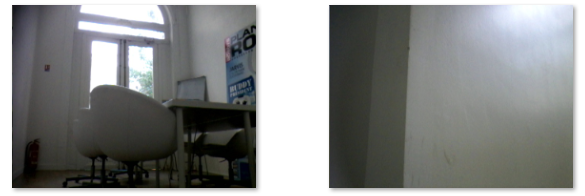
\includegraphics[width=0.8\linewidth]{img/wall.png}
  \caption{Comparison of a normal image (left) who has 1392 keypoints detected, and a wall image (right) who has only 10. The BRISK detector is used.}
\label{wall}
\end{figure}
% image comparison of information rich and poor images
In Figure \ref{wall} we show an image taken facing a wall and another normal image.
In the tests, wall often cause problems for the robot's navigation, and there
are in general two cases. In the first case, the robot faces a wall. As 
there are no nearly keypoints to identify, and the robot is unable to find an
orientation. This case can occur rather often, especially in corridors, thus 
degrading the performance. While in the second case, the robot can, following an imprecise orientation, advance toward a wall and bump into it. Although this is not very dangerous, but it is evidently better to avoid such collisions. 

\subsubsection{Wall Detection}
To detect walls, we can use the Canny edge detector, who finds edges in the image along with their intensity. In addition, its computation is 5 to 20 times faster than the detection of keypoints according to the tests. 

\begin{figure}[h]
\centering
  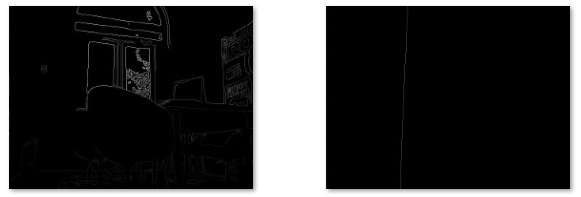
\includegraphics[width=0.8\linewidth]{img/wall_canny.png}
  \caption{Two images in Figure \ref{wall} after processed by the Canny edge detector}
\label{wall_canny}
\end{figure}

Figure \ref{wall_canny} shows the same two images transformed with the Canny edge detector. We can see that in the normal image there are much more white pixels which correspond to edges. If we count the number of these non-zero valued pixels, there is a significant difference: 13734 for the first image and 963 for the second. Therefore we can use this metric to detect walls.

Consequently for each new image taken during navigation, we can first run this wall detection algorithm before the rather costly keypoint detection and descriptor calculation algorithm. This can avoid much unnecessary calculation. On the other hand, after certain orientation results, we may use wall detection to verify that there is no wall before the robot and it can safely advance. 
% TODO: problem of distance: how to we distinguish the case when there is a wall at the end of the corridor and it is safe to advance / the case where the wall is just in front of the robot?

\subsubsection{Orientation Adjustment}
Once we have detected a wall during a navigation process, we have the possibility to adjust directly the advancing direction. To achieve this goal, we split the image into three vertical slices of equal width. Then we run the wall detection algorithm separately in the left, center and right part of the image. If we detected a wall on the left-hand side, we turn to the right; if there are walls on two sides, we go direct ahead; if walls are present in all three sections, the robot could turn 180 degrees, etc.

\subsubsection{Potential Difficulties}
As we don't have the depth information, there can exist some problematic cases:
\begin{enumerate}
    \item Textured wall. When there is a textured wall or obstacle, it will not be detected. Therefore it is necessary to use other kind of sensor information.
    \item Distant wall. Even if the way is far away, the robot may still detect it and refrain from advancing.
\end{enumerate}

\subsubsection{Infrared Sensors}
In addition to vision, infrared sensors can provide us with useful information for wall detection. 

% TODO: change the name of saliency
\subsection{Saliency Test}
\begin{figure}[H]
\centering
\begin{minipage}{0.33\textwidth}
  \centering
  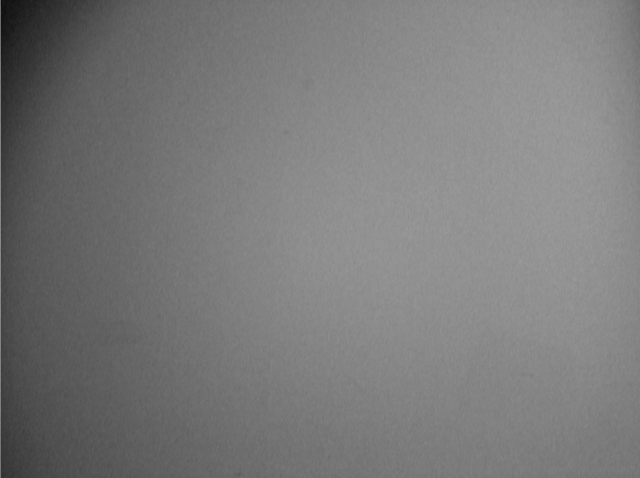
\includegraphics[width=0.9\linewidth]{img/walldetect.png}
  \caption{Wall}
  \label{suptrain}
\end{minipage}%
\begin{minipage}{0.33\textwidth}
  \centering
  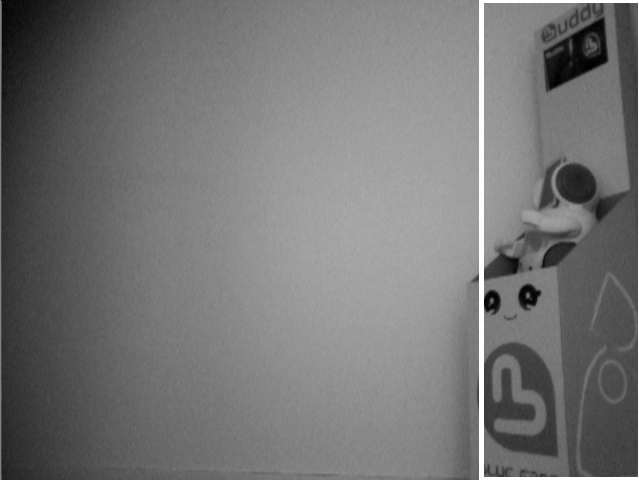
\includegraphics[width=0.9\linewidth]{img/saliency.png}
  \caption{Partially wall}
  \label{states_sup}
\end{minipage}
\begin{minipage}{0.33\textwidth}
  \centering
  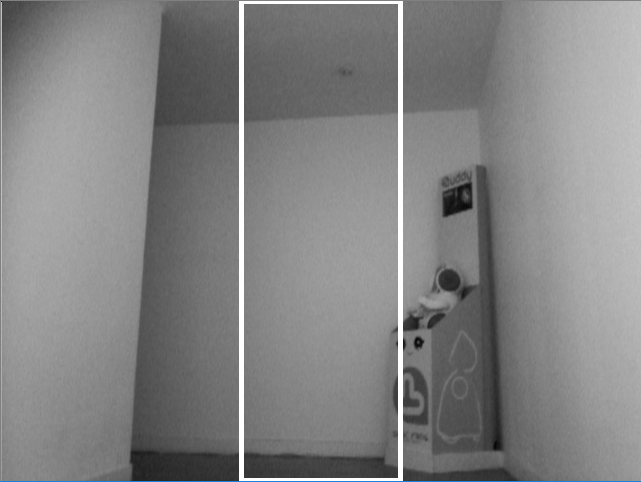
\includegraphics[width=0.9\linewidth]{img/corridor.png}
  \caption{Center of corridor}
  \label{states_sup}
\end{minipage}

\end{figure}


\subsubsection{Two-stage orientation with salience shifting}
In order to overcome these potential shortcomings, as well as to integrate wall detection into the existing orientation method, we have conceived the following two-stage algorithm. 

%http://www.texample.net/tikz/examples/simple-flow-chart/


%TODO: to modify this!!!
\begin{figure}
    \centering
    \caption{Two-stage orientation algorithm}
    \vskip 8pt
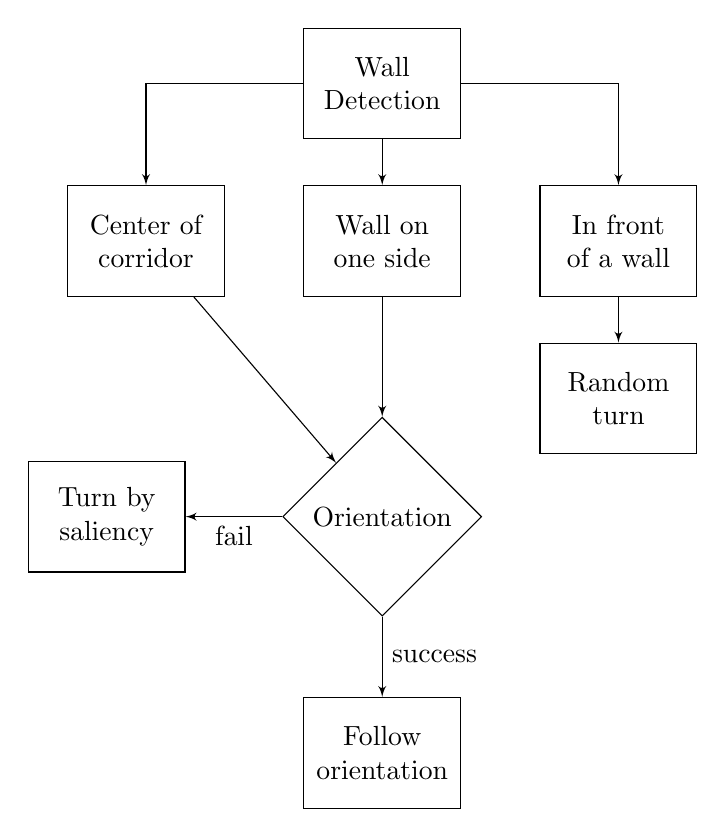
\begin{tikzpicture}[node distance = 2cm, auto]
    % Place nodes
    \node [block] (init) {Wall Detection};
    \node  [block, below of=init](side) {Wall on one side};
    \node [block, left of=side, node distance=3cm] (corridor) {Center of corridor};
    \node  [block, right of=side, node distance=3cm](wall) {In front of a wall};
    \node [block, below of=wall] (random) {Random turn};
    \node [decision, below of=side, node distance = 3.5cm] (go1){Orientation};
    \node [block, left of =go1, node distance = 3.5cm](turn) {Turn by saliency};
    \node [block, below of=go1, node distance = 3cm](follow) {Follow orientation};
    
    \path [line] (init) -| (wall);
    \path [line] (init) -| (corridor);
    \path [line] (init) -- (side);
    \path [line] (side) -- (go1);
    \path [line] (wall) -- (random);
    \path [line] (corridor) -- (go1);
    \path [line] (go1) -- node {success} (follow);
    \path [line] (go1) -- node {fail} (turn);
\end{tikzpicture}
    \label{algo_orientation}
\end{figure}

% simpler version


\subsection{Ground obstacles}
As the field of view of the camera is rather limited, the obstacles on the floor are often not taken in the photos. Therefore, we can instead use the infrared sensors to detect obstacles.

\subsection{Mobile obstacle}

% TODO: organize visual obstacle avoidance and X

% TODO: A global navigation 

% And this works!

\section{Programming Skills}
During the internship, I have also gained more experience in programming.

Vision-related navigation and localization algorithms are principally written in \ttt{C++} in order to use libraries like OpenCV. I got to become familiarized with some basic features of modern \ttt{C++} (\ttt{C++11} and \ttt{C++14}):

\begin{enumerate}
\item \ttt{auto} specifier. use automatic type deduction can save a lot of typing.
\item for loop comprehension.
\item lambda functions.
\item \ttt{std::map}
\item shared and unique pointers.
\end{enumerate}


\newpage
\printbibliography
\end{document}

